The kinematic tree is an abstract representation of a collection of transforms. 
Unlike the rigid collection (section \ref{sec: rigid}), the kinematic tree is able to represent transforms in multiple datum frames. 
The tree can then use the network of frames to "lookup" a transform between any two connected nodes, as hinted at in figure \ref{fig: poses}.
This concept is widely used in robotics and therefore has a place in the prototyping package. 
There are several algorithms this class implements:
\begin{enumerate}
	\item Representation: Construct a tree representation given only the edges
	\item Lookup: apply breadth first graph search to find a path between any two nodes on the tree
	\item Root: use depth first search to express all frames in the base link frame or another specified frame on the tree
\end{enumerate}

\subsection{Representation}
Frames in a kinematic tree must have a child frame, a parent frame, or both. 
Frame $T$ is described as:
\begin{equation}
	T_i^{p(i)} = \begin{bmatrix}
		R_i^{p(i)} & t_i^{p(i)} \\
		\bf{0} & 1
	\end{bmatrix}
\end{equation}
where $i$ is the child frame, and $p(i)$ is the parent frame. 
The kinematic tree has a root, which we can also call the "base link". 
The challenge with the kinematic tree is that we are only given the transforms, which are the edges in the graph. 
So we need to create a tree representation from just the transforms. 
Transforms contain the parent and child of the edge, and are therefore directed. 
Thus we want a representation that is easily able to express the directed nature of the graph. 

The importance of the edges in the kinematic tree suggests that an incidence list is the best representation for this situation. 
For example, say we have a tree as shown in figure \ref{fig: tree}.

\begin{figure}
	\centering
	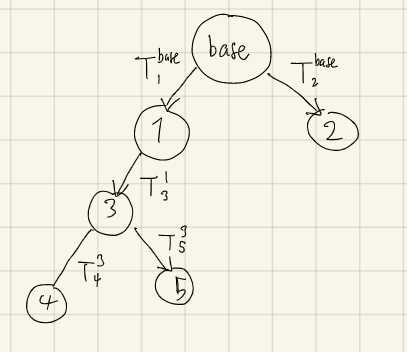
\includegraphics[width=0.5\textwidth]{images/example_tree.png}
	\caption{Example tree}
	\label{fig: tree}
\end{figure}

This takes the form:
\begin{align}
	base &: \big[ T^{base}_1, T^{base}_2\big] \\
	1 &: \big[ T^1_3, T^1_{base} \big]\\
	2 &: \big[ T^2_{base}\big]\\
	3 &: \big[ T_4^3, T_5^3 \big] \\
	4 &: \big[ T_3^4\big] \\
	5 &: \big[ T_3^5\big] \\
\end{align}
We can improve memory storage by using a dictionary (hash map) in order to only save the relevant edges. 
The construction algorithm is shown in algorithm \ref{alg: inc_list}.

\begin{algorithm}
	\DontPrintSemicolon
	\KwIn{Unordered edge set $T$}
	\KwOut{Hash map where frames are the keys and the transforms they are incident with are values}
	tree $\gets \{\}$

	\tcp{hash.insert(key : value)}
	tree.insert(root : $\varnothing$)

	\For{$t \in T$}{$p \gets t.parent$

		$c \gets t.child$

		\tcp{process parents first}
		\If{$p \neq NULL$}{
			\eIf{$p \in$ tree}{
				\tcp{we store list of transforms touching $p$}
				tree[$p$].append($t$)
			}{
				tree.insert($p : \varnothing$)
			}
		}

		\tcp{process children}
		\If{$c \neq NULL$}{
			\eIf{$c \in $ tree}{
				\tcp{store whether the edge is forwards (used later)}
				($t^{-1}).forwards \gets false$

				tree[$c$].append($t^{-1}$)
			}{
				tree.insert($c : \varnothing$)
			}

		}
	}

	\Return{tree}
	\caption{Incidence list representation for the Kinematic Tree}
	\label{alg: inc_list}
\end{algorithm}

Once the incidence list is constructed, then we can use it to query the tree to find paths between frames.
The incidence list can keep track of the direction by assigning a flag to each edge specifying whether it is backwards or forwards. 
This will be useful for the rooting algorithm, shown later. 

An important thing to note is that in the context of the kinematic tree, an edge transform $T^i_j$ contains a child $j$ and a parent $i$ similar to a node. 
However an edge can only have one parent and one child, whereas a node can have only one parent, but many children. 

\subsection{Lookup path between frames}

Now say we wanted to know the transform between two frames $i, j$ on the tree that aren't connected by an existing edge. 
We can find this edge, $T_i^j$ by finding the path between the two frames, and then multiplying the transforms we pass through, as shown in figure \ref{fig: lookup}.

\begin{figure}
	\centering
	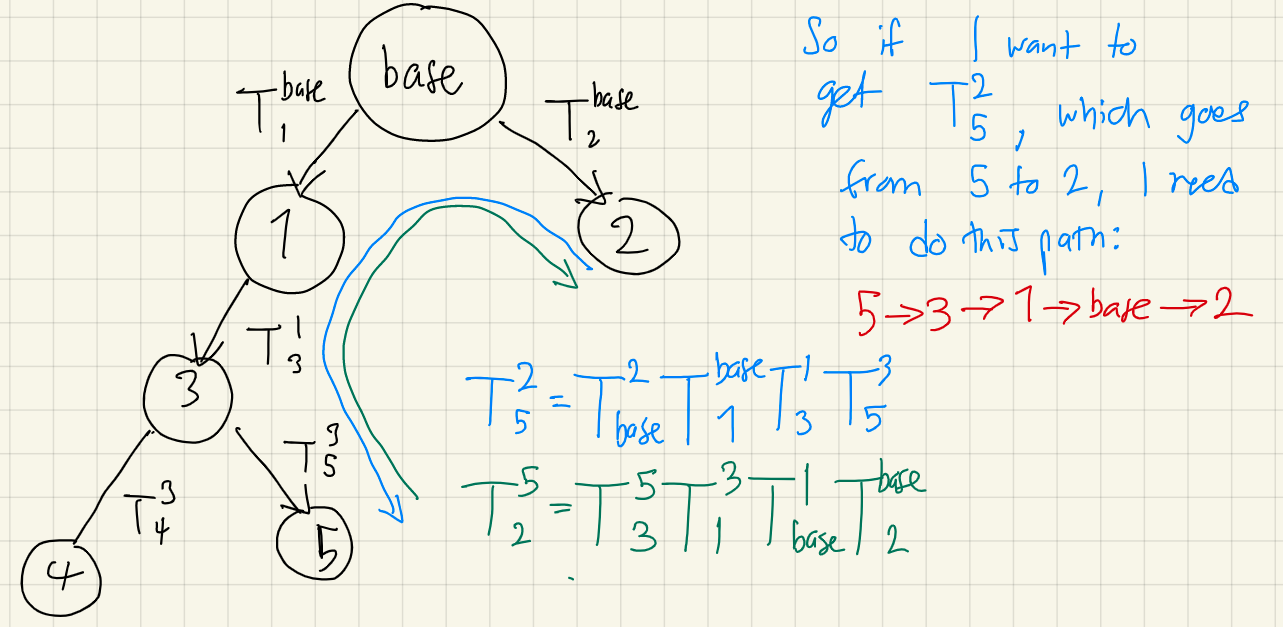
\includegraphics[width=\textwidth]{images/lookup_path.png}
	\caption{Lookup path between frames}
	\label{fig: lookup}
\end{figure}

This can be done by executing a breadth first search on the tree in an attempt to find a path between two frames. 
The algorithm is given in alorithm \ref{alg: lookup}.
The algorithm shows how the algorithm is modified to deal with the need to store edges. 
Once we have a path as a sequence of edges, we can multiply these transforms together to obtain the transform between frames $i, j$.


\begin{algorithm}
	\KwIn{start frame, end frame}
	\KwOut{backpointers dictionary}
	\DontPrintSemicolon
	\SetKwFunction{expand}{expand}
	\SetKwFunction{bfs}{search\_for\_path}
	\SetKwProg{Fn}{def}{:}{}	$O \gets \varnothing$

	\tcp{the main search function}
	\Fn{\bfs{$x_{start}, x_{goal}$}}{

		$C \gets \varnothing$

		\tcp{the backpointers dictionary stores edges we've passed through}
		backpointers = \{\}

		$O$.insert(start)

		backpointers.insert(start:$NULL$)

		\While{$O \notin \varnothing$}{
			$x \gets O$.pop()

			$C$.insert($x$)

			\If{\expand{x}}{
				\Return{Success, backpointers}
			}

	}

	\Return{Failure, backpointers}
	}	

	\tcp{The node expansion function}
	\Fn{\expand{x}}{
		\tcp{get the ordered set of transforms linked to $x$}
		$T \gets x.edges$

		\For{
			$t \in T$
		}{

			\uIf{$t$.child = end}{
				backpointers.insert($t.child : t$)
				
				\Return{Success}
				}
			\ElseIf{$t.child \notin O \textrm{ and } t.child \notin C$}{

				backpointers.insert($t.child : t$)

				O.insert($t.child$)
			}
			
			\Return{Failure}
			
		}
	}

	\caption{Lookup between frames using breadth first search. The backpointers can then be used to extract the path of $n$ transforms between the frames: $\prod_i^n T_i^{p(i)}T^i_{c(i)}$}
	\label{alg: lookup}
\end{algorithm}

\subsection{Root function}
The other main algorithm used by the kinematic tree is the root function. 
The purpose of this is simply to put every frame in the tree into the base frame. 
From here, it is trivial to place the entire tree in coordinates of any frame in the tree. 
If we use figure \ref{fig: lookup} for reference, then we want the frames $T^{base}_1,T^{base}_2, T^{base}_3, T^{base}_4, T^{base}_5$.
We can obtain this through a depth first search that visits nodes in order and extracts the transform during the traversal. 
Using the tree in figure \ref{fig: lookup}, we would visit the nodes from left to right: 4, 3, 5, 1, 2. 

\begin{algorithm}
	\SetKwFunction{expand}{expand}
	\SetKwProg{Fn}{def}{:}{}	$O \gets \varnothing$

	\KwIn{Root of the tree}
	\KwOut{Dictionary of transforms $T_i^{base}$ for each frame $i$ in the tree}

	frames = \{\}

	$O \gets \varnothing$

	$C \gets \varnothing$

	$O$.insert(root)

	\While{$O \neq \varnothing$}{
		$x \gets O$.pop
		
		$C$.insert($x$)

		\expand{x}

	}

	\Return{frames}

	\tcp{depth first search expansion}
	\Fn{\expand{$x$}}{
		\tcp{traverse the ordered set $T$ of neighboring edges in reverse order}

		$R \gets reverse(T)$

		\ForAll{$t \in R$}{
			\If{$t.forward()$}{
				$x \gets t.child$

				$p \gets t.parent$

				\If{$x \notin O and x \notin C$}{
					$O$.insert($x$)

					$t^p_x \gets $ frames[$p$]

					frames.insert($x$ : $t^{p}_x$ * $t$)
				}
			}
		}
	}

	\caption{The depth first traversal used to derive the set of transforms $\mathcal{T} =\{ T^{base}_i \forall i : i \in K\}$ with frames $i$ in kinematic tree $K$.}
	\label{alg: root}
\end{algorithm}

This is shown in algorithm \ref{alg: root}. 
The root function can then be used to graph the entire tree in the base frame or any other frame in the tree. 